\documentclass{beamer}

\usetheme[hideothersubsections]{Berkeley}

% these are typical

\usepackage{latexsym}		% to get LASY symbols
\usepackage{epsfig}		% to insert PostScript figures
\usepackage{graphicx}           % to insert any other kind of figure

% these are for math stuff

\usepackage{amsmath}	% AMS math features (e.g., eqn alignment)
\usepackage{amssymb}	% Various weird symbols
\usepackage{amsfonts}	% Various useful math fonts
\usepackage{amsthm}	% Fancy theorem-type environments

% Uncomment these lines to make full-size pages for printing
%\usepackage{pgfpages}
%\pgfpagesuselayout{resize to}[letterpaper,border shrink=5mm,landscape]

% {definition}, {example}, {examples}, {lemma}, {theorem}, and {fact}
% already defined
\newtheorem{question}{Question}
\newtheorem{conjecture}{Conjecture}

\begin{document}

\raggedright

\title{A Question Answering System Using Encoder-decoder Sequence-to-sequence Recurrent Neural Networks}
\author{Bo Li}
\date{May, 2018}
\institute[SJSU]{San Jos\'{e} State University}

\begin{frame}
\titlepage

\end{frame}

\begin{frame}

  \frametitle{Outline}

  \tableofcontents[hideallsubsections]

\end{frame}



\section{Introduction}

\begin{frame} \frametitle{Question Answering}
    \begin{itemize}
        \item is the study of writing computer programs that can answer natural language questions
        \item is widely used among search engines, personal assistant applications on smart phones, voice control systems and various other applications
        \item  can be categorized into two types - open domain and close domain
            \begin{itemize}
                \item  For an open domain system, the questions can be about almost everything.
                \item For a close domain system, the questions are about a specific domain.
            \end{itemize}
    \end{itemize}
\end{frame}


\begin{frame}{Topic of This Project}
    \begin{itemize}
        \item open domain
        \item a scenario where a specific passage is already assigned to a question and the answer is a segment of the passage
        \item The Stanford Question Answering Dataset (SQuAD) used in this project is appropriate for such scenario
            \begin{itemize}
                \item includes questions asked by human beings on Wikipedia articles
                \item The answer to each question is a segment of the corresponding Wikipedia passage
                \item contains more than 100,000 question-answer pairs on more than 500 articles
            \end{itemize}
    \end{itemize}
\end{frame}

\begin{frame}{Encoder-decoder Sequence-to-sequence Recurrent Neural Networks}
   \begin{itemize}
       \item Encoder-decoder:  encode an input to some vectors and then decode those vectors to an output.
       \item Sequence-to-sequence: Input is a sequence; output is also a sequence
            \begin{itemize}
                \item For question answering, the input sequence includes a passage and a question and the output sequence is the answer
            \end{itemize}
       \item Recurrent Neural Networks: Networks used for modeling sequential data

   \end{itemize}
\end{frame}

\begin{frame}{Contribution of This Project}
    \begin{itemize}
        \item We successfully built a question answering system using five different models
        \item By comparing the results of five different models, we got two interesting observations
    \end{itemize}
\end{frame}

\section{Background}

\begin{frame} \frametitle{Word Feature Vector}\framesubtitle{Overview}
  \begin{itemize}
      \item A word feature vector represents a word according to its relationship with other words in a vocabulary.
      \item The distance from one word feature vector to any other word feature vector tells how likely the two words appear in a same context.
      \item The word feature vector matrix for the vocabulary of a given text are learned by training a neural probabilistic language model on the text.
  \end{itemize}
\end{frame}

\begin{frame}{Word Feature Vector, cont.}\framesubtitle{Neural Probabilistic Language Model}

    \begin{itemize}
        \item Some notations
            \begin{itemize}
                \item V: vocabulary
                \item $w_t$: as a word from $V$
                \item $C$: the matrix which includes the word feature vectors of all words in $V$
            \end{itemize}
        \item Each instance of the training set is a sequence of words $w_t, ..., w_{t-n+1}$ which is a segment of the text.
        \item The purpose of a neural probabilistic language model is to learn a model $f$ such that
        $$ f(w_t, ..., w_{t-n+1}) = \hat{P}(w_t | w_{t-1},...,w_{t-n+1}).$$
    \end{itemize}
\end{frame}

\begin{frame}{Word Feature Vector, cont.}\framesubtitle{Neural Probabilistic Language Model}
    \begin{itemize}
        \item The computation of $f(w_t, ..., w_{t-n+1})$ is divided into two parts:
            \begin{itemize}
                \item First, each $w$ is mapped to a word feature vector by selecting the corresponding row in $C$ to get

                $$x=(C(w_{t-1}),... ,C(w_{t-n+1})).$$

                \item Second, we get $f(w_t, ..., w_{t-n+1})$ through

                $$y=b+W\cdot x + U\cdot tanh(d + H\cdot x)$$

                and

                $$ f(w_t, ..., w_{t-n+1}) = \frac{e^{y_{w_t}}}{\sum_{i}^{}e^{y_i}}.$$
            \end{itemize}
        \item The loss function to minimize is $$L = -\frac{1}{T}\sum _{t}^{} \log{f(w_t, ..., w_{t-n+1})}.$$
    \end{itemize}
\end{frame}

\begin{frame}{Word Feature Vector, cont.}\framesubtitle{Usage in This Project}
   \begin{itemize}
       \item In this project, we used the word feature vectors to represent words.
   \end{itemize}

\end{frame}
\begin{frame}{Recurrent Neural Networks}\framesubtitle{Overview}

Recurrent Neural Networks (RNNs) are used for modeling sequential data.

    \begin{examples}{A simple recurrent network with no outputs.}
        \begin{itemize}
            \item $x$ is the input. $h$ is the state. $\theta$ is the hyperparameter.
            \item The relation between $h$ and $x$ is
            $$h_t = f(h_{t-1}, x_t; \theta).$$
                \begin{center}
                  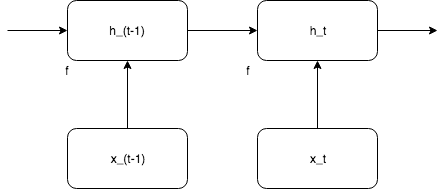
\includegraphics[width=5cm, height=2cm]{figures/rnnWithNoOutputs}
                \end{center}
            \item An example of $f$ is $h_t = sigmoid(W_h h_{t-1} + W_x x_t + b).$
        \end{itemize}

    \end{examples}
\end{frame}


\begin{frame}{Recurrent Neural Networks, cont.}\framesubtitle{Long Short Term Memory (LSTM) cell}
    \begin{itemize}
        \item Vanishing gradient problem
            \begin{itemize}
                \item the vanishing gradient means the gradients become smaller and smaller as their values are propagated forward in a network
                \item When this happens, the network learns slowly or even stops learning
            \end{itemize}
        \item The main solution to the vanishing problem: Use a more complex learning unit
        \item Long Short Term Memory (LSTM) cell is one such complex learning unit; Gated Recurrent Unit (GRU) has a simplified structure but similar function with LSTM
    \end{itemize}
\end{frame}

\begin{frame}{Recurrent Neural Networks, cont.}\framesubtitle{Usage in This Project}
    \begin{itemize}
        \item In this project, we used LSTM and GRU equally as learning unit.
    \end{itemize}
\end{frame}

\begin{frame}{Bidirectional Recurrent Neural Networks}\framesubtitle{Overview }
    \begin{itemize}
        \item Problem of RNNs: $h_t$ only contains context information from $x_1$ to $x_t$
        \item Solution given by Bidirectional RNNs:
            \begin{itemize}
                \item one cell operates from left to right, and another cell operates from right to left
                \item using both $h_t$ and $g_t$ can get context information of the whole sequence
            \end{itemize}
             \begin{center}
                  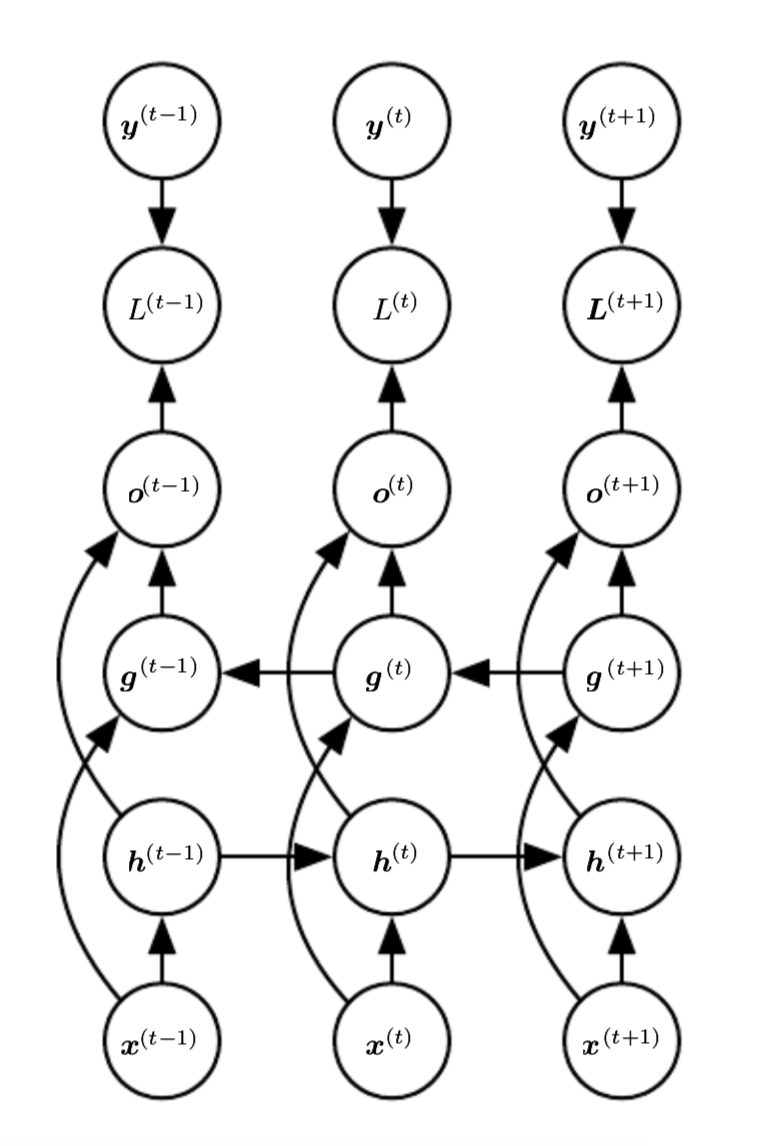
\includegraphics[width=8cm, height=4cm]{figures/bidirectionalRnn.png}
            \end{center}
    \end{itemize}
\end{frame}

\begin{frame}{Bidirectional Recurrent Neural Networks}\framesubtitle{Usage in This project}
    \begin{itemize}
        \item In this project, we used bidirectional RNNs in encoding part.
    \end{itemize}
\end{frame}

\begin{frame}{Encoder-decoder Sequence-to-sequence Architecture}
\begin{itemize}
    \item The process of understanding the input sequence is considered as encoding the input sequence to some vectors $Crypto$.
    \item The process of generating output is considered as decoding the $Crypto$.
\end{itemize}

\begin{examples}
$x$ is the input, $h$ is the state in encoding process, $y$ is the output, and $g$ is the state of decoding process.
\end{examples}

\end{frame}

\begin{frame}{Encoder-decoder Sequence-to-sequence Architecture, Cont.}
    \begin{center}
        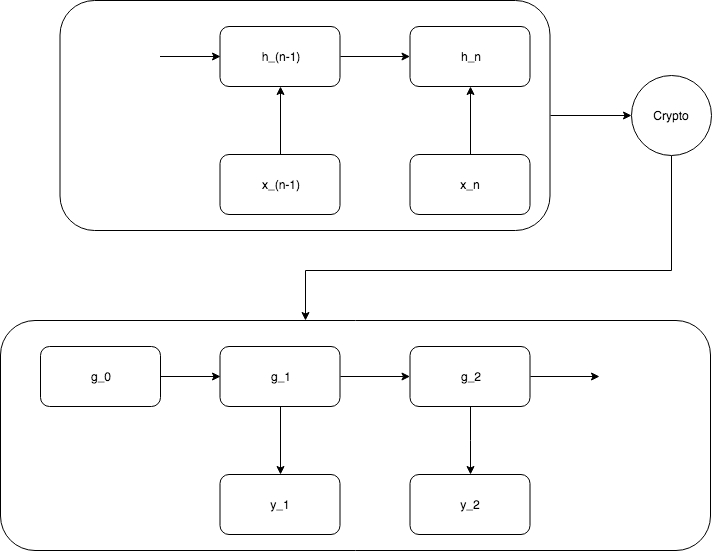
\includegraphics[width=10cm, height=7cm]{figures/encoderDecoder.png}
    \end{center}
\end{frame}

\begin{frame}{Encoder-decoder Sequence-to-sequence Architecture, Cont.}
    \begin{itemize}
        \item The question answering task in this project is a sequence-to-sequence task.
        \item Each input actually includes two sequences - a question and a passage.
            \begin{itemize}
                \item attention mechanism is required to make each passage aware of the corresponding question and encode the two together
            \end{itemize}
        \item each output sequence is an answer which is represented by two indices for the input passage sequence.
            \begin{itemize}
                \item pointer network is required to make sure the output sequence comes from input sequence
            \end{itemize}
    \end{itemize}

\end{frame}

\begin{frame}{Attention Mechanism}
    \begin{itemize}
        \item first used in neural machine translation
        \item is used to enable the decoding process aware of the encoding states
    \end{itemize}
\end{frame}

\begin{frame}{Attention Mechanism, Cont.}
    \begin{examples}
        $y$ is the output, $g$ is the state, and $c$ is the attention vector. $$g_i =f(g_{i-1},y_{i-1},c_i).$$
        The attention vector $c_i$ is produced by using $g_{i-1}$ to ``query'' the encoding states $h_1, ... h_n$ through
        $$c_i = \sum _j {\alpha _{i,j} h_j}$$
        $$\alpha _{i,j} = \exp{e_{i,j}} / \sum _j {\exp{e_{i,j}}}$$
        $$e_{i,j} = tanh(W_h h_j + W_g g_{i-1} + b).$$
    \end{examples}

\end{frame}

\begin{frame}{Attention Mechanism, Cont.}
    \begin{center}
        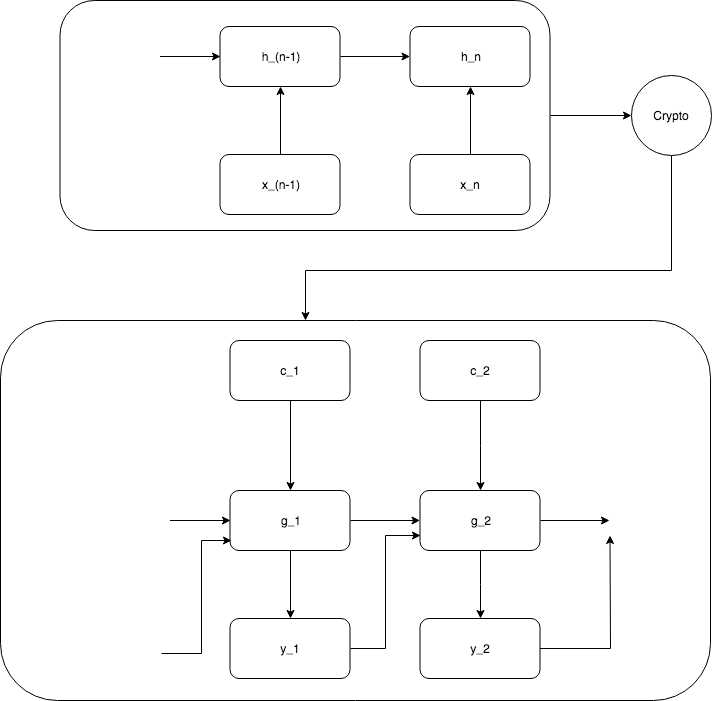
\includegraphics[width=8cm, height=8cm]{figures/attention}
    \end{center}
\end{frame}

\begin{frame}{Attention Mechanism, Cont.}
    In this project, the passage is required to ``be aware of the question'' in encoding process. At the same time, the answer is required to ``be aware of the encoding states of passage and question''. The detailed formulas are given later.
\end{frame}

\begin{frame}{Pointer Network}
    \begin{itemize}
        \item Using the pointer network enables the decoder to output tokens from input sequence
        \item The attention mechanism is used with the pointer network
        \item However, aside from getting an attention vector, the attention weight vector $\alpha$ is considered as a probability distribution which indicates how likely each token in the input sequence is the current output.
        $$y_i = x_k$$
        where
        $$k = argmax_j(\alpha _{i,j}).$$
    \end{itemize}
\end{frame}

\begin{frame}{Pointer Network, Cont.}
    \begin{center}
        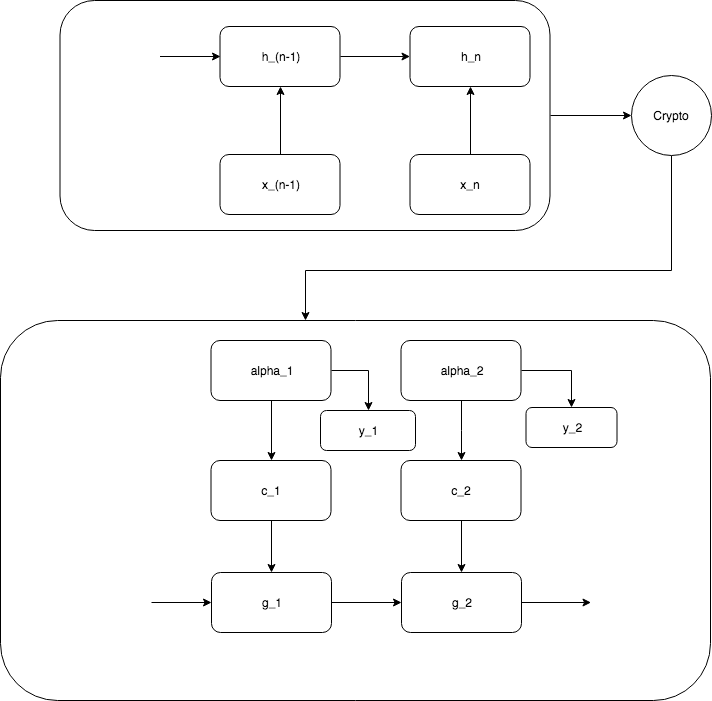
\includegraphics[width=8cm, height=8cm]{figures/pointerNetwork.png}
    \end{center}

\end{frame}

\begin{frame}{Pointer Network, Cont.}
    In this project, the pointer network was used in the decoding part of several models.
\end{frame}
\section{Design}

\begin{frame}{}
    In this chapter, I will explain the five models one by one. Recall that Model 1 is the Match LSTM \& Answer Pointer model which has a typical encoder-decoder sequence-to-sequence recurrent network architecture designed by Wang and Jiang. Model 2, 3, 4 and 5 are designed by making changes to Model 1.
\end{frame}

\begin{frame} \frametitle{Model 1}
  \begin{itemize}
      \item an encoder-decoder sequence-to-sequence architecture
      \item on SQuAD dataset.Each instance of training data includes one passage, one question and one answer. The passage is a sequence of tokens, the question is a sequence of tokens, and the answer is a sequence of two indices indicating the start and end positions in passage.
      \item Before feeding training data into the model, tokens in passages and questions are vectorized to word feature vectors.
  \end{itemize}
\end{frame}

\begin{frame} \frametitle{Model 1, cont.}\framesubtitle{Structure Overview}
    \begin{itemize}
        \item Encoder
            \begin{itemize}
                \item the preprocessing layer
                \item the bidirectional match LSTM layer
            \end{itemize}
        \item Decoder
            \begin{itemize}
                \item the answer pointer layer
            \end{itemize}
    \end{itemize}

\end{frame}

\begin{frame} \frametitle{Model 1, cont.}\framesubtitle{the preprocessing layer}

    \begin{itemize}
        \item a LSTM runs over each passage word feature vector sequence and outputs a sequence of LSTM states
        \item The same LSTM is used to encode each question word feature vector sequence to a sequence of LSTM states.
    \end{itemize}
\end{frame}

\begin{frame} \frametitle{Model 1, cont.}\framesubtitle{the preprocessing layer}
    $$H^p = \overrightarrow{LSTM}(P)$$
    $$H^q = \overrightarrow{LSTM}(Q)$$

    where

    $$P\in R^{d \times p}: passage$$
    $$Q\in R^{d \times q}: question$$
    $$H^p\in R^{l \times p}: encoded\ passage$$
    $$H^q\in R^{l \times q}: encoded\ question$$
    $$p: length \ of\ passage$$
    $$q: length\ of\ question$$
    $$l: dimension\ of\ LSTM\ states$$
    $$d: dimension\ of\ word\ feature\ vector$$

\end{frame}

\begin{frame} \frametitle{Model 1, cont.}\framesubtitle{bidirectional match LSTM layer}

a LSTM equipped with passage-question attention, which is called match LSTM, is used to encode each sequence of passage states and the corresponding sequence of question states together to a sequence of match LSTM states.


\end{frame}

\begin{frame} \frametitle{Model 1, cont.}\framesubtitle{bidirectional match LSTM layer}

    $$\overrightarrow{G} = tanh(W^qH^q + (W^p{h_i}^p + W^r\overrightarrow{{h_{i-1}}^r} + b^p) \otimes e_q)$$
    $$\overrightarrow{\alpha _i} = softmax(w^t\overrightarrow{G_i} + b \otimes e_q)$$


    where

    $$W^q, W^p, W^r\in R^{l \times l} $$
    $$b_p, w\in R^{l}  $$
    $$b \in R $$
    $${h_{i}^p}\in R^{l}: one\ column\ of\ H^p  $$

    and

    \[ \overrightarrow{z_i} =
    \begin{bmatrix}
    {h_i}^p \\
    H^q\overrightarrow{ {\alpha _i}}^T \\
    \end{bmatrix}
    \in R^{2l}
    \]
    $$\overrightarrow{{h_i}^r} = \overrightarrow{LSTM}(\overrightarrow{z_i}, \overrightarrow{{h_{i-1}}^r}).$$

\end{frame}

\begin{frame} \frametitle{Model 1, cont.}\framesubtitle{bidirectional match LSTM layer}
    After iterating between getting attention weight vector $\overrightarrow{\alpha _i}$ and getting match LSTM state ${{h_{i}}^r}$ $p$ times, we get $[{{h_{1}}^r}, ..., {{h_{p}}^r}]$. Concatenate them to get

    $$\overrightarrow{H^r} = [{{h_{1}}^r}, ..., {{h_{p}}^r}] \in R^{l \times p}.$$

    Then go over $H^p$ from right to left to get $\overleftarrow{H^r}$. Concatenate $\overrightarrow{H^r}$ and $\overleftarrow{H^r}$ to get the final output of encoding process

    \[ H^r =
    \begin{bmatrix}
    \overrightarrow{H^r} \\
    \overleftarrow{H^r} \\
    \end{bmatrix}
    \in R^{2l \times p}.
    \]
\end{frame}

\begin{frame} \frametitle{Model 1, cont.}\framesubtitle{answer pointer layer}
each output of the decoding process includes two probability distributions.
   \begin{itemize}
       \item The first probability distribution tells how likely each token in passage to be the start of the answer.
       \item The second probability distribution tells how likely each token in passage to be the end of the answer
   \end{itemize}
\end{frame}

\begin{frame}\frametitle{Model 1, cont.}\framesubtitle{answer pointer layer}
    $$F_k = tahn(VH^r + (W^a{h^a_{k-1}} +  b^a) \otimes e_p)$$
    $$\beta _k = softmax(v^tF_k + c \otimes e_p)$$


    where
    $$V \in R^{l \times 2l}$$
    $$W^a\in R^{l \times l} $$
    $$b_a, v\in R^{l}  $$
    $$c \in R $$
    $${h_{k-1}}^a\in R^{l}: ith\ state\ of\ answer\ LSTM  $$

    and answer LSTM is


    $${h_k}^a = LSTM(H^r\beta _k^T, h_{k-1}^a)$$
\end{frame}

\begin{frame}\frametitle{Model 1, cont.}\framesubtitle{answer pointer layer}
    By iterating between the attention mechanism and the answer LSTM two times, we could get the output of the decoding process - $\beta _0$ and $\beta _1$.


    Now we can get the loss function. Let $a_s$ denote the ground truth start index of the answer and $a_e$ denote the ground truth end index, we have

    $$p(a|H^r) = p(a_s|H_r)p(a_r|H_r)=\beta _{0, a_s} \times \beta_{1, a_e}$$

    where $$\beta_{k, j} = jth\ token\ of\ \beta _k$$

\end{frame}

\begin{frame}\frametitle{Model 1, cont.}\framesubtitle{loss function}
    To train the model, the loss function

    $$J(\theta) = -\frac{1}{N}\sum_{i=1}^{N} \log{p(a^n|H^r)} $$

    is minimized.
\end{frame}

\begin{frame} \frametitle{Model 2}
    The difference from Model 2 and Model 1 is in the decoding process. In Model 2,
    $${h_k}^a = H^r\beta _{k}^T.$$
    That is, instead of the current state of answer LSTM, the previous attention vector is used to query the current attention weight vector.
\end{frame}

\begin{frame} \frametitle{Model 3}
    The difference between Model 3 and Model 2 is that in Model 3 the $W^r\overrightarrow{{h_{i-1}}^r}$ in the bidirectional match LSTM layer is removed. This modification aims at checking whether $\overrightarrow{{h_{i-1}}^r}$ carries some redundant context information. After this change,


    $$\overrightarrow{G} = tanh(W^qH^q + (W^p{h_i}^p + b^p) \otimes e_q)$$
\end{frame}

\begin{frame} \frametitle{Model 4}
    The difference between Model 4 and Model 2 is that in Model 4 the the preprocessing layer is removed. This modification aims at checking whether the preprocessing layer carries some redundant context information.
\end{frame}

\begin{frame} \frametitle{Model 5}
    The difference between Model 5 and Model 2 is that in Model 5 both the preprocessing layer and $W^r\overrightarrow{{h_{i-1}}^r}$ in the bidirectional match LSTM layer are removed. This aims at checking whether context information carried by both is included in some other parts of Model 2.
\end{frame}

\section{Implementation}

\begin{frame} \frametitle{Adjusting Models for Batch Training}\framesubtitle{Why necessary?}
    \begin{itemize}
        \item When training a model, all of the training data is fed into the model to update the parameters.
        \item In one specific model, the number of times to iterate the encoding process is fixed.
        \item However, different passages have different lengths and different questions also have different lengths.
        \item As such, adjusting all passages to a same length and adjusting all questions to another same length are necessary.
    \end{itemize}
\end{frame}

\begin{frame}\frametitle{Adjusting Models for Batch Training}\framesubtitle{How to pad?}
    For sequences longer than a fixed length, a part of the sentence is cut out. For sequences shorter than a fixed length, a faking pad token is used to pad them. In practice, each passage is adjusted to $passage\_padding\_length$ and is paired with a mask vector $passage\_mask$ which has size $passage\_padding\_length$. Each question is adjusted to $question\_padding\_length$ and paired with a mask vector $question\_mask$ which has size $question\_padding\_length$. Each entry of mask vector is either zero or one. Zero indicates that the current token does not exist in the original sequence. One indicates the opposite.
\end{frame}
\begin{frame}\frametitle{Adjusting Models for Batch Training}\framesubtitle{Take Model 1 as an example}
    In the preprocessing layer, after getting a sequence of states, the mask vector is used to reset the values of positions that do not exist to zero in an additional step
    $$H^p = H^p \circ (passage\_mask \otimes l)$$
    $$H^q = H^q \circ (question\_mask \otimes l).$$
    In the match LSTM layer, the attention weights of positions that do not exist are also set to zero in an additional step
    $$\overrightarrow{\alpha _i} = softmax( (w^t\overrightarrow{G_i} + b \otimes e_q) ) \circ question\_mask .$$
    Similar to the preprocessing layer, we have
    $$H_r = H_r \circ (passage\_mask \otimes 2l).$$
    In the answer pointer layer, similar to the match LSTM layer, we have
    $$\beta _k = softmax( (v^tF_k + c \otimes e_p) ) \circ passage\_mask.$$


\end{frame}

\begin{frame}{Tensorflow Graphs}
    \begin{itemize}
        \item Tensorflow is an open source machine learning framework.
        \item The central idea of Tensorflow is describing a complex numeric computation as a graph.
        \item {\tt Variables} are ``trainable'' nodes.
        \item {\tt Placeholders} are nodes whose values are fed in run time.
    \end{itemize}
\end{frame}

\begin{frame}{Tensorflow Graphs}\framesubtitle{Taking Model 1 as an example}
     \begin{itemize}
         \item {\tt Variables} should be used to represent all the parameters of the encoding and decoding layers
         \item {\tt Placeholders} should be used to represent passages, questions, and answers.
         \item To train a graph, some APIs of Tensorflow are called to get a train operation.
         \item Then the training data is fed through {\tt Placeholders} to run the train operation. When the train operation is run, the {\tt Variables} are updated.
     \end{itemize}
\end{frame}

\begin{frame}{Tensorflow Graphs}\framesubtitle{Taking Model 1 as an example}
    \begin{center}
        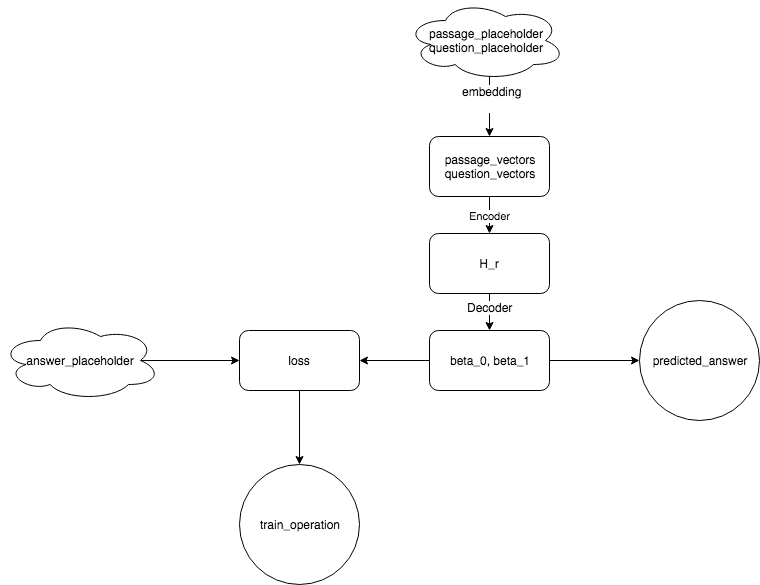
\includegraphics[width=8cm, height=6cm]{figures/tf_graph.png}
    \end{center}
\end{frame}

\begin{frame}{Implementation Pipeline}
    \begin{itemize}
        \item For a specific model, in the train and validation process, some Tensorflow graphs that have same structure but different values for {\tt Variables} are saved.
        \item The validation loss is used to choose the best graph. Then the best graph is used to do testing.
    \end{itemize}
    \begin{center}
      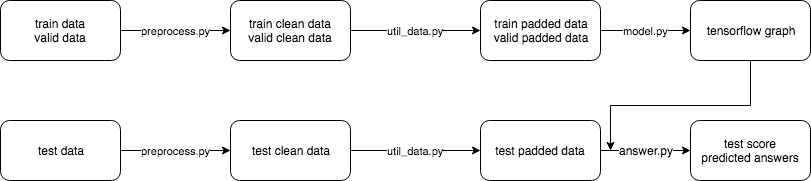
\includegraphics[width=9cm, height=2.5cm]{figures/pipeline.png}
    \end{center}
\end{frame}

\section{Experiments}

\begin{frame} \frametitle{Data}
    \begin{itemize}
        \item The Stanford Question Answering Dataset (SQuAD) is used to do experiments.
        \begin{table}[htbp]\centering
          \begin{tabular}{|r|l|} \hline
            Set Name & Number of Instances \\ \hline\hline
            Train & \ 78,839 \\
            Validation & \ 8,760 \\
            Test & \ 10,570 \\ \hline
          \end{tabular}
        \end{table}
        \item The pre-trained GloVe word feature vectors are used to initialize words.
    \end{itemize}
\end{frame}

\begin{frame}\frametitle{Data}
    \begin{center}
        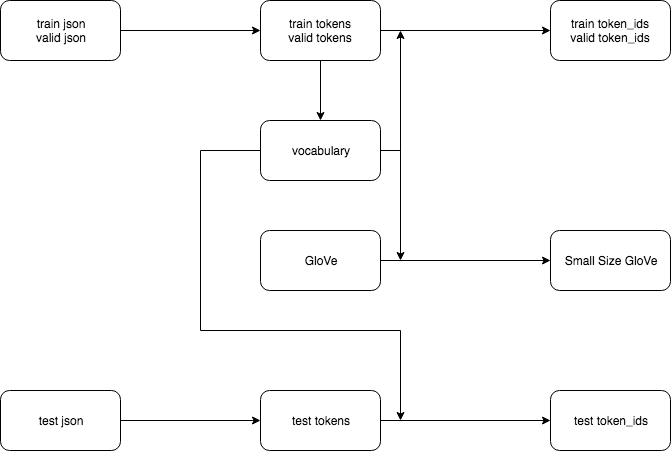
\includegraphics[width=8cm, height=6cm]{figures/data.png}
    \end{center}
\end{frame}

\begin{frame}{Settings}
    \begin{itemize}
        \item 400 is set as $passage\_padding\_length$
            \begin{center}
                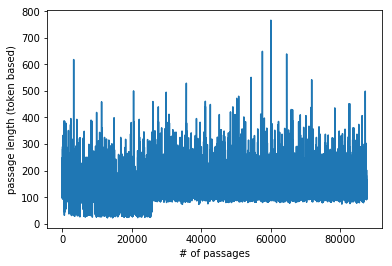
\includegraphics[width=6cm, height=4cm]{figures/passage_length.png}
            \end{center}
    \end{itemize}
\end{frame}

\begin{frame}{Settings}
    \begin{itemize}
        \item 30 is set as $question\_padding\_length$
            \begin{center}
                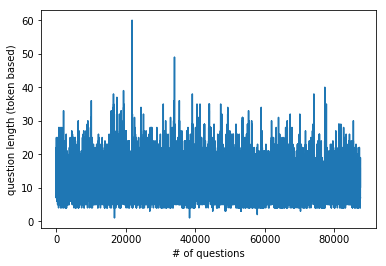
\includegraphics[width=6cm, height=4cm]{figures/question_length.png}
            \end{center}
    \end{itemize}
\end{frame}

\begin{frame}{Settings}
    \begin{itemize}
        \item The learning rate is set at 0.002 through experiments.
    \end{itemize}
    \begin{center}
        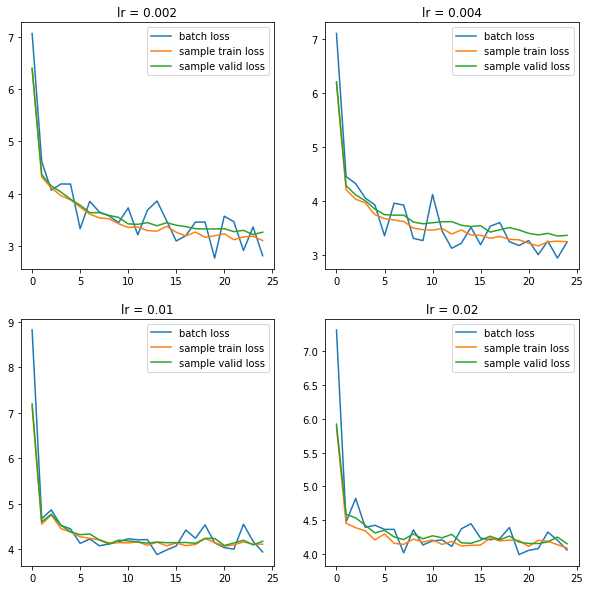
\includegraphics[width=7cm, height=7cm]{figures/lr.png}
    \end{center}
\end{frame}

\begin{frame}{Settings}
    \begin{table}[htbp]\centering

      \begin{tabular}{|r|l|} \hline
        Hyperparameter Name& Value \\ \hline\hline
        Word Feature Vector Dimension (d) & \ 100 \\
        Hidden State Size (l) & \ 64 \\
        L2\_regularization Scale & \ 10570\\
        Hidden State Size (l) & \ 64\\
        Batch Size & \ 64\\
        Passage Length & \ 400\\
        Question Length & \ 30\\
        Clip Norm & \ 5\\
        Learning Rate & \ 0.002 \\ \hline
      \end{tabular}
    \end{table}
\end{frame}

\begin{frame}{Settings}
    \begin{itemize}
        \item The F1 score and the exact match score are used to evaluate the performance of each model.
            \begin{itemize}
                \item F1 treats a predicted answer and a ground truth as bag of words and calculate a harmonic average of precision and recall;
                \item exact match measures the percentage of predictions and ground truths that are exactly the same. The testing data contains several ground truth answers for one passage-question pair. The best score is chosen as the final score.
            \end{itemize}
        \item A machine that has Tesla K80 12 GB Memory, 61 GB RAM and 100 GB SSD is used to train the models.
    \end{itemize}
\end{frame}

\begin{frame}{Training Process}
    \begin{itemize}
        \item One epoch contains roughly 25 * 100 mini batches.
        \item The training loss and training scores are calculated every 100 mini batches using the 200 sample instances from training set. We do the same for validation loss and validation scores.
        \item Training one epoch takes roughly 100 minutes. A thorough training of each model requires around 10 epochs and takes around 17 hours.
    \end{itemize}
\end{frame}

\begin{frame}{Training Process}\framesubtitle{Model 1}
    \begin{center}
        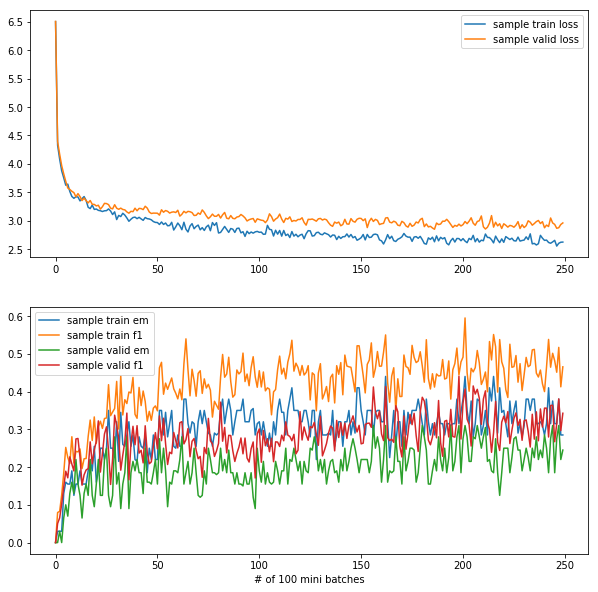
\includegraphics[width=8cm, height=7cm]{figures/match_corrected.png}
    \end{center}

\end{frame}

\begin{frame}{Training Process}\framesubtitle{Model 2}
    \begin{center}
        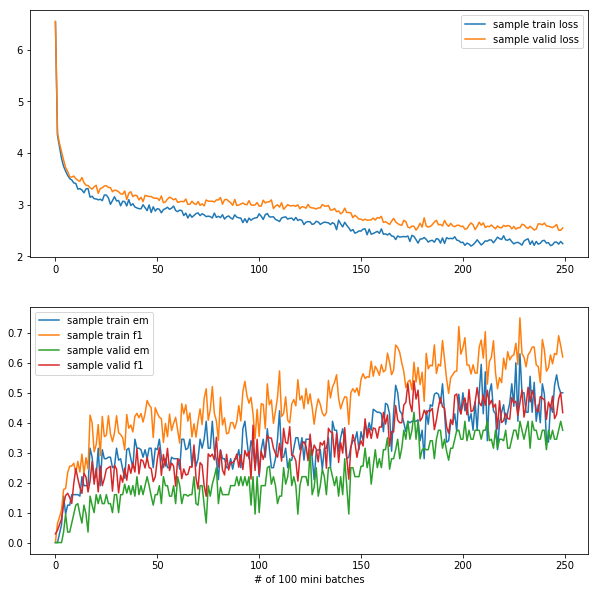
\includegraphics[width=8cm, height=7cm]{figures/match_baseline.png}
    \end{center}
\end{frame}

\begin{frame}{Training Process}\framesubtitle{Model 3}
    \begin{center}
        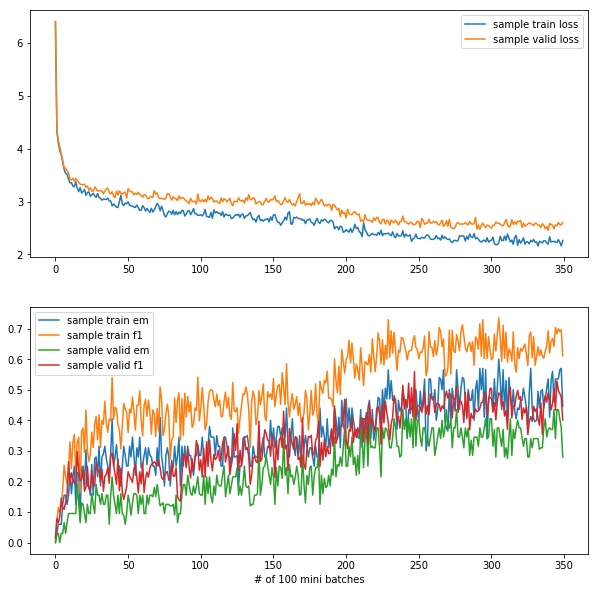
\includegraphics[width=8cm, height=7cm]{figures/match_change1.png}
    \end{center}

\end{frame}

\begin{frame}{Training Process}\framesubtitle{Model 4}
    \begin{center}
        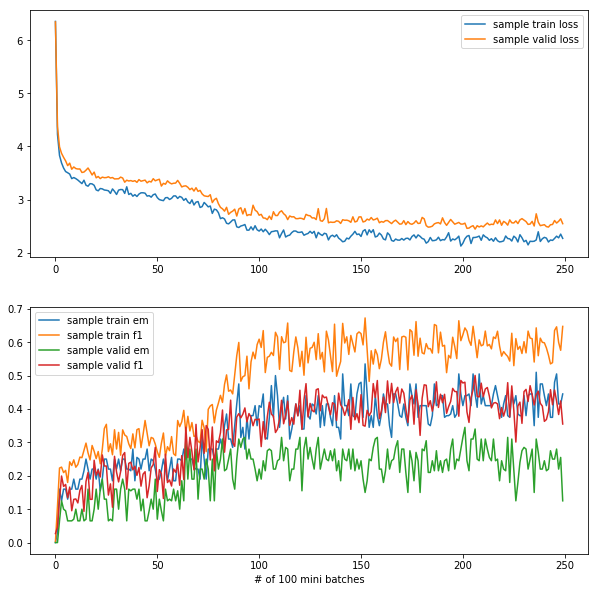
\includegraphics[width=8cm, height=7cm]{figures/match_change2.png}
    \end{center}

\end{frame}

\begin{frame}{Training Process}\framesubtitle{Model 5}
    \begin{center}
        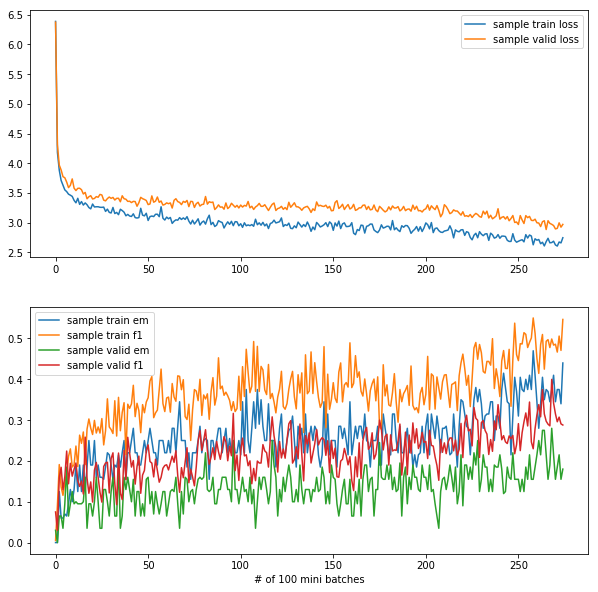
\includegraphics[width=8cm, height=7cm]{figures/match_change3.png}
    \end{center}

\end{frame}

\begin{frame}{Testing Results}
    \begin{table}[htbp]\centering
      \caption{Testing results}
      \label{tab:test_results}
      \begin{tabular}{|c|c|c|}
        \hline
        Model& Test Exact Match & Test F1 \\
        \hline\hline
        Model 1 & \ 23.4 &\ 33.6 \\
        Model 2 & \ 33.0 &\ 45.8 \\
        Model 3 & \ 33.0 &\ 46.2 \\
        Model 4 & \ 33.0 &\ 45.6 \\
        Model 5 & \ 24.3 &\ 33.9 \\
        \hline
      \end{tabular}
    \end{table}
\end{frame}

\begin{frame}{Analysis}
    \begin{itemize}
        \item Model 1 didn't reproduce the results of the original paper.
        \item Comparing the testing results of Model 2 and Model 1, the scores of Model 2 are better.  Model 2 uses previous attention vector to query the current attention weight vector. However, Model 1 uses the current answer LSTM state to query the attention weight vector. The answer LSTM state is produced by applying a non-linear transformation on the attention vector. It turns out not including the non-linear transformation gives better results.
    \end{itemize}
\end{frame}

\begin{frame}{Analysis}
    \begin{itemize}
        \item Model 2, 3 and 4 behave similarly. This means removing either the preprocessing layer or the $h_r$ in the bidirectional match LSTM layer does not decrease test results. A reasonable guess is the two parts provide duplicate context information.

        \item Model 5 performs worse than Model 2, 3 and 4. This means removing both the preprocessing layer and the $h_r$ in the bidirectional match LSTM layer decreases testing results. A reasonable guess is the context information provided by these two parts is not provided in other parts of Model 1. As such, one of the two must be kept.
    \end{itemize}
\end{frame}

\section{Conclusion}

\begin{frame}{Contribution of This Project}
    \begin{itemize}
        \item This project presented a thorough implementation of a question answering system. \item Five different models were tried and several interesting observations were found.
    \end{itemize}

\end{frame}

\begin{frame} \frametitle{Future Work}
    \begin{itemize}
        \item Further work is required to find out why Model 1 failed to reproduce the testing results of the reference paper.
        \item At the same time, more parameter tuning work is required to make the experiments more precise. \item Last but not the least, making novel architectures to bypass the state-of-art results is always a good way to move the question answering research forward.
    \end{itemize}
\end{frame}

\begin{frame}
Thank you! Questions?
\end{frame}

\end{document}
